\chapter{SAMBA 4}

O software Samba 4 vem com a proposta de criar um substituto livre para o \textit{Active Directory}, combatendo as versões pagas da Microsoft, utilizando o LDAP, Bind (ou um DNS interno que o próprio Samba 4 possui) e Kerberos. Esta versão vem com a intenção de ser uma evolução do Samba 3. Com o Samba 4 o administrador de rede é capaz de fornecer na rede serviços como, controle de usuários, máquinas, compartilhamento de arquivos, compartilhamento de impressoras, controle de acesso ao compartilhamento e entre outros.
Com a adoção de um \textit{Active Directory} no mesmo sistema que fornece o compartilhamento de arquivos e impressoras, o Samba 4 permite uma ligação nas configurações de permissões a usuários inseridas no compartilhamento com os usuários cadastrados no domínio, assim eliminando a divisão entre o servidor de domínio e o de compartilhamento.

O sistema ainda esta em desenvolvimento mas já passou por todas as suas fases de testes iniciais alpha e beta, atualmente esta na 4º Release Candidate, mas sem data para o lançamento da versão estável.

\section{Instalação do SAMBA 4}

Todos os comandos foram testados no Ubuntu 11.04 e Debian 6, por isso algumas adaptações podem ser necessárias em outras distribuições Linux.

A instalação é realizada a partir do terminal, mas antes é necessária a instalação de algumas bibliotecas.

\begin{itemize}
	\item \textbf{\# apt-get install build-essential libattr1-dev libblkid-dev libgnutls-dev python-dev git-core autoconf python-dnspython ntpdate acl libacl1-dev}
\end{itemize}

Antes de começar a instalação o relógio do servidor tem que estar atualizado. O comando ntpdate atualiza a hora através do  ntp\footnote[2]{Os servidores NTP permitem aos seus clientes a sincronização dos relógios de seus computadores e outros equipamentos de rede a partir de uma referência padrão de tempo aceita mundialmente, conhecida como UTC (\textit{Universal Time Coordinated}).\cite{RNP}} , onde um dos principais servidores é o pool.ntp.br.

\begin{itemize}
	\item \textbf{\# ntpdate pool.ntp.br}
\end{itemize}

O código fonte do Samba 4 esta hospedado no servidor git dos desenvolvedores do Samba, e o mesmo deve ser clonado para a maquina de destino.

\begin{itemize}
	\item \textbf{\# git clone git://git.samba.org/samba.git samba-master; cd samba-master}
\end{itemize}

O Samba 4 segue os procedimento padrões de instalação de aplicativos no Linux através do terminal que, segundo \cite{INSTALL}, se segue com o ./configure, make e o make install. Nesse caso ao invés de se utilizar o ./configure como padrão é utilizado o ./configure.developer, pois o mesmo habilita alguns modos de debug.

\begin{itemize}
		\item \textbf{\# ./configure.developer}
		\item \textbf{\# make}
		\item \textbf{\# make install}
\end{itemize}

Para verificar a versão instalada é só executar o seguinte comando:

\begin{itemize}
	\item \textbf{\# /usr/share/local/samba/bin/smbclient "--version}
\end{itemize}

\section{Criação de Domínio com o Samba 4}

O Samba 4 trabalha com regras ACL e, para que ele possa ser instalado, deve-se habilitar o modo acl nas unidades de disco.

\begin{itemize}
	\item \textbf{\# vim /etc/fstab}
\end{itemize}

Deve-se localizar a linha da unidade principal (/) e adicionar o parâmetro acl na coluna options da montagem desta unidade, conforme figura \ref{fstab}.

\begin{figure}[ht]
   	\centering
    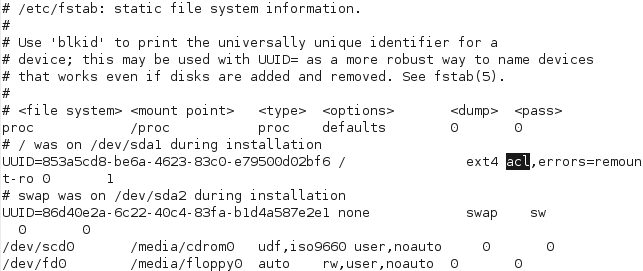
\includegraphics[width=0.8 \textwidth]{figuras/fstab}
   	\caption{Tela do fstab.}
    \label{fstab}
\end{figure}
 
\pagebreak

Por padrão o Samba 4 é instalado no /usr/local/samba.

\begin{itemize}
	\item \textbf{\# cd /usr/local/samba}
\end{itemize}

A instalação do Samba 4 é realizada através do samba-tools, uma ferramenta que acompanha o Samba 4, que fica localizado na pasta bin do Samba 4. Deve-se usar as opções ``domain provision" e após inserir alguns parâmetros importantes para a configuração do domínio, conforme comando abaixo. Os parâmetros serão detalhados a seguir.

\begin{itemize}
	\item \textbf{\# bin/samba-tool domain provision "--use-ntvfs "--realm=iff.bomjesus  \\"--domain=iff  "--adminpass=`Senha12' "--server-role=dc}
\end{itemize}

\begin{enumerate}
	\item \textbf{use-ntvfs} - Habilita o NTVFS\footnote[3]{Sistema de arquivos que armazena os atributos do NTFS};
	\item \textbf{realm} - Domínio do servidor Kerberos;
	\item \textbf{domain} - Domínio do Samba;
	\item \textbf{adminpass} - Senha do Administrator, por questões de segurança o samba-tool não permite a inserção de senhas consideradas fracas como senhas com menos de 7 dígitos e somente com números em sequência;
	\item \textbf{server-role} - Regra do servidor.
\end{enumerate}

Depois de instalado e configurado o Samba 4 pode ser iniciado.

\begin{itemize}
	\item \textbf{\# /usr/local/samba/sbin/samba -i -M single}
\end{itemize}

Para facilitar a forma de ativar o Samba 4 podem ser feito dois procedimentos.

Criar um link do executável do Samba no /etc/init.d/

\begin{itemize}
	\item \textbf{\# ln /usr/local/samba/sbin/samba /etc/init.d/samba}
\end{itemize}

Mudar o caminho da variável de ambiente PATH para que os comandos possam ser acessados fora da sua pasta de origem.

\begin{itemize}
	\item \textbf{\# echo ``export PATH=/usr/local/samba/sbin:/usr/local/samba/bin:\$PATH" $>$$>$ \\ /root/.bashrc}
\end{itemize}

Por padrão o Samba 4 vem com uma servidor interno de DNS, facilitando a criação das zonas e dos mapeamentos. Para a resolução dos nome deve definir o ip da própria maquina como seu dns primário. Cabe resaltar que os micros clientes do domínio devem ser configurados para usar o servidor do Samba 4 como DNS primário.

\begin{itemize}
	\item \textbf{\# echo ``domain iff nameserver 192.168.0.1" $>$ /etc/resolv.conf}
\end{itemize}

Mesmo contendo um servidor de dns interno o Samba 4 também trabalha com servidores externos, BIND9 versão 9.7 ou mais nova, onde alguns parâmetros de configuração são passados no named.conf.local e named.conf.options para a criação das zonas e atualização automática com o Kerberos.

\begin{itemize}
	\item \textbf{\#echo ``include `/usr/local/samba/private/named.conf'" $>$ /etc/bind/named.conf.local}
	\item \textbf{\# vim /etc/bind/named.options}
\end{itemize}

Adicione as seguintes linhas contidas no Quadro \ref{named_options}:\\

\begin{lstlisting}[caption=Arquivo named.options,label={named_options}]
options{ 
	
directory '/usr/local/bind/var/run/named'; 

tkey-gssapi-keytab '/usr/local/samba/private/dns.keytab'; 

tkey-domain 'iff.bomjesus';
	
};
\end{lstlisting}

As variáveis adicionadas no arquivos são para:

\begin{itemize}
	\item{directory} -  É o caminho absoluto do seu servidor dns;
	\item{tkey-gssapi-keytab} - Local da chave do dns para conexão com o kerberos;
	\item{tkey-domain} - Nome do Domínio.
\end{itemize}

\section{Instalação do Kerberos}

Segundo \citeonline{HEIMDAL} a autenticação Kerberos é um protocolo de rede. Foi concebido para fornecer autenticação forte para o cliente/servidores de aplicativos usando criptografia de chaves secretas, então um cliente pode provar a sua identidade para um servidor (e vice-versa) em uma conexão de rede insegura.Em nosso caso utilizaremos o Heimdal Kerberos por causa do GSS-TSIG algoritmo de serviço de segurança genérico para autenticação de transação com chave secreta de DNS (GSS-TSIG) este mecanismo é utilizado para estabelecer relações TSIG para autenticação do tipo Kerberos, com essas credenciais o DNS aceita atualizações GSS-TSIG assinadas e verifica as credenciais de correspondentes com as credencias cadastradas no Samba 4, isso permite aos usuários descarregar o DNS dos usuários do Microsoft Windows sem ter a segurança comprometida.

\begin{itemize}
	\item \textbf{\# apt-get install krb5-user krb5-kdc krb5-config kstart} - Instala todos os pacotes necessários e faz as referências necessárias.
\end{itemize}

Após instalar os pacotes, substitua-se o /etc/krb5.conf pelo arquivo criado e pré-configurado pelo Samba que esta localizado em /usr/local/samba/private/krb5.conf .

\begin{itemize}
	\item \textbf{\# cp /usr/local/samba/private/krb5.conf  /etc/}
\end{itemize}

Teste para verificar se todos as configurações foram realizadas corretamente.

\begin{itemize}
	\item \textbf{\# host -t SRV \_ldap.\_tcp.IFF.BOMJESUS.} - O resultado deve ser parecido : \textbf{\_ldap.\_tcp.IFF.BOMJESUS has SRV record 0 100 389 server.``nome do realm sem aspas".}
	\item \textbf{\# host -t SRV \_kerberos.\_udp.IFF.BOMJESUS.} - O resultado deve ser parecido : \textbf{\_kerberos. \_udp.IFF.BOMJESUS has SRV record 0 100 88 server.IFF.BOMJESUS.}
	\item \textbf{\# host -t A IFF.BOMJESUS} - O resultado deve ser parecido : \textbf{IFF.BOMJESUS has address 192.168.0.1.} 
\end{itemize}

\section{Gerenciando o Samba4 através do Windows e do Linux}

É possível gerenciar o servidor Samba 4 através de um Windows XP mas para a realização do mesmo é necessário a instalação do AdminPack\footnote[4]{O AdminPack está disponível no site da Microsoft:

http://www.microsoft.com/downloads/details.aspx?FamilyID=c16ae515-c8f4-47ef-a1e4-a8dcbacff8e3\&displaylang=en} presente no Windows Server. Essa ferramenta permite gerenciar todos os usuários, grupos e máquinas presentes no \textit{Active Directory}

Inicie a ferramenta pelo \textbf{Executar -$>$ dsa.msc} - Figura \ref{dsa} e o programa já executado como pode ser visto na Figura \ref{tela_dsa}.

\begin{figure}[ht]
   	\centering
    \scalebox{1}{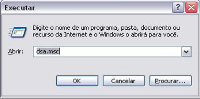
\includegraphics{figuras/dsamsc}}
   	\caption{Tela para executar o DSA.}
    \label{dsa}
\end{figure}
 
\begin{figure}[h!]
   	\centering
    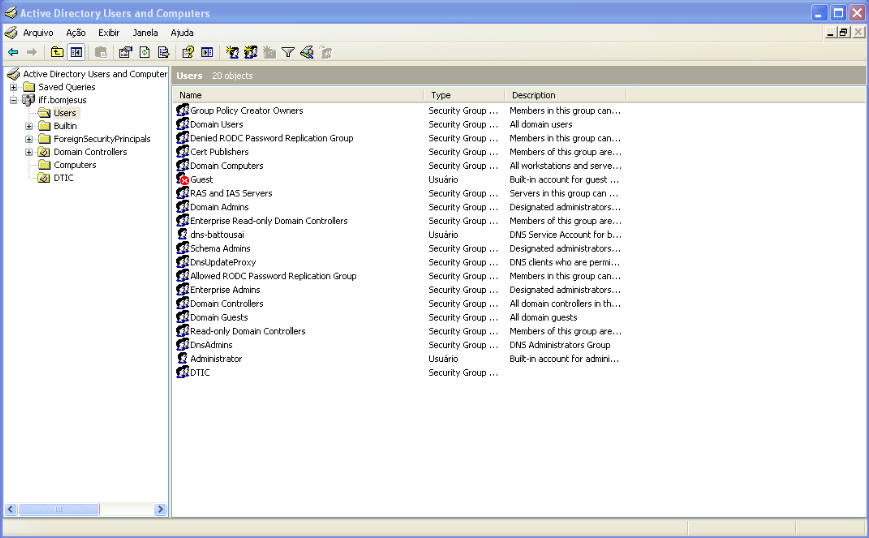
\includegraphics[width=0.7 \textwidth]{figuras/addsa}
   	\caption{Tela do DSA.}
    \label{tela_dsa}
\end{figure}

Outra forma de gerenciar o servidor Samba 4 é utilizando o samba-tools, uma ferramenta que acompanha o Samba 4 e tem a finalidade de gerenciar as ações que podem ser feitas no no \textit{Active Directory}. Com ele se poder criar usuários, grupos, gpo's, entre outras funções, porém através do terminal do Linux, conforme Figura \ref{samba-tool}.

\pagebreak

\begin{figure}[ht]
   	\centering
    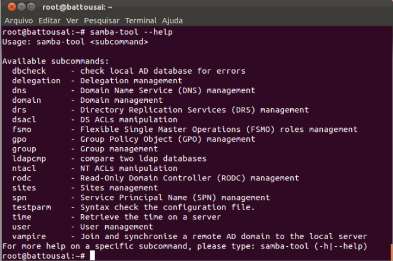
\includegraphics[width=0.7 \textwidth]{figuras/samba-tool}
   	\caption{samba-tool no terminal.}
    \label{samba-tool}
\end{figure}

\section{Máquinas Linux interagindo com o \textit{Active Directory} do  Samba4}

A forma de incluir uma maquina Ubuntu no \textit{Active Directory} é modificar alguns arquivos de configuração. A seguir será apresentado um passo-a-passo para inclusão do Ubuntu no domínio \cite{UBUNTU-WIKI}. Segue abaixo os procedimentos descritos na \textit{Wiki} do Ubuntu.

Para tal, foi utilizado como exemplo de configuração do domínio as seguintes informações:

Descrição das variáveis que serão utilizadas na configuração e seus valores.

\begin{itemize}
	\item \textbf{fja.br} -  Domínio do \textit{Active Directory}.
	\item \textbf{fjadc01.fja.br} - Controlador de domínio.
	\item \textbf{10.1.0.1} - IP do controlador de domínio.
	\item \textbf{FJA.BR} - Kerberos Realm.
	\item \textbf{gert} - Estação de Trabalho Ubuntu.
	\item \textbf{gert.fja.br} - FQDN da estação de trabalho.
	\item \textbf{fjadc01} - Servidor NTP.
\end{itemize}

\begin{enumerate}
	\item \textbf{Instalando os pacotes necessários}
\begin{itemize}
	\item \textbf{\# aptitude install krb5-user libpam-krb5 winbind samba smbfs smbclient krb5-config libkrb53 libkadm55 vim}
\end{itemize}

	\item \textbf{Sincronizando a hora}

\begin{itemize}
	\item \textbf{\# ntpdate 10.2.0.1} 
\end{itemize}

	\item \textbf{Edite o arquivo /etc/hosts adicionando o ip e o nome do DC de sua rede. Exemplo no Quadro \ref{hosts}.}
	\begin{itemize}
			\item \# vim /etc/hosts\\
	\end{itemize}
		\begin{lstlisting}[caption=Valores que devem ser adicionados no /etc/hosts,label={hosts}]
127.0.0.1       gert.fja.br localhost gert

127.0.1.1       gert

# The following lines are desirable for IPv6 capable hosts

::1     ip6-localhost ip6-loopback

fe00::0 ip6-localnet

ff00::0 ip6-mcastprefix

ff02::1 ip6-allnodes

ff02::2 ip6-allrouters

ff02::3 ip6-allhosts

10.2.0.1   fjadc01

10.2.0.2   fjadc02

\end{lstlisting}

	\item \textbf{Configurando o Kerberos}
		\begin{itemize}
			\item {\# vim /etc/krb5.conf} - Edite o arquivo conforme o exemplo do Quadro \ref{krb5}.\\
		\end{itemize}
		\begin{lstlisting}[caption=Valores que devem ser adicionados no /etc/krb5.conf,label={krb5}]
[libdefaults]

default_realm = FJA.BR

[realms]

FJA.BR = {

kdc = fjadc01.fja.br

default_domain = FJA.BR

kpasswd_server = fjadc01.fja.br

admin_server = fjadc01.fja.br

}

[domain_realm]

.fja.br = FJA.BR
\end{lstlisting}

	\item \textbf {Testando a conexão com o \textit{Active Directory}.}
		\begin{itemize}
			\item {kinit $<$ENTER$>$}
			\item {Password for alex$@$FJA.BR: ****}
			\item {klist $<$ENTER$>$}
			\item {Ticket cache: FILE:/tmp/krb5cc\_1000}
			\item {Default principal: alex$@$FJA.BR}
		\end{itemize}

	\item \textbf {Se o resultado for igual a do Quadro \ref{kerberos_ok} o Kerberos está funcionando corretamente.}\\

		\begin{lstlisting}[caption=Resultado se o Kerberos esta funcionando perfeitamente.,label={kerberos_ok}]
Valid starting Expires Service principal 07/16/07 15:48:35  
07/17/07 01:49:08  

krbtgt/FJA.BR@FJA.BR renew until 07/17/07 15:48:35
	
Kerberos 4 ticket cache: /tmp/tkt1000
	
klist: You have no tickets cached
\end{lstlisting}

	\item \textbf{Acessando o Domínio.}
		\begin{itemize}
			\item {\# vim /etc/samba/smb.conf} -  Adicione as linhas contidas no Quadro \ref{smb_conf}.\\
		\end{itemize}

		\begin{lstlisting}[caption=Arquivo smb.conf para fazer \textit{login} em um domínio.,label={smb_conf}]
[global]

security = ads
		
realm = FJA.BR

password server = 10.2.0.1

workgroup = ADMINISTRATIVO

idmap uid = 10000-20000

idmap gid = 10000-20000

winbind enum users = yes

winbind enum groups = yes

template homedir = /home/\%D/\%U

template shell = /bin/bash

client use spnego = yes

client ntlmv2 auth = yes

encrypt passwords = yes

winbind use default domain = yes

restrict anonymous = 2

# to avoid the workstation from

# trying to become a master browser

# on your windows network add the

# following lines

domain master = no

local master = no

preferred master = no

os level = 0
\end{lstlisting}

	\item \textbf{Reinicie os serviços.}
	
			1. \# /etc/init.d/winbind stop
			
			2. \# /etc/init.d/samba restart
			
			3. \# /etc/init.d/winbind start

	\item \textbf{Adicione a conta ao domínio.}\\
		\begin{itemize}
			\item \# net ads join
		\end{itemize} 
		\begin{itemize}
			\item \textbf{Resultado} - Using short domain name – GERT Joined ``GERT" to realm ``FJA.BR"
		\end{itemize}

	\item \textbf{Configure a Autenticação.}
		\begin{itemize}
				\item {\# vim /etc/nsswitch.conf} - Adicione as linhas contidas no Quadro \ref{nsswitch_conf}.\\
		\end{itemize}
		\begin{lstlisting}[caption=Arquivo /etc/nsswitch.conf,label={nsswitch_conf}]
passwd:   compat winbind

group:    compat winbind

shadow:   compat
		\end{lstlisting}

 	\item \textbf{Teste o winbind}
		\begin{itemize}
			\item {getent passwd}
		\end{itemize}
		quiosque:*:10018:10000:Quiosque:/home/ADMINISTRATIVO/quiosque:/bin/bash

		\begin{itemize}
			\item {getent group}
		\end{itemize}

		\_\_coordenação de enfermagem:x:10046:coordenf

		\_\_coordenação de design:x:10047:smarino,coorddes

	\item \textbf{Configure o PAM.}
		\begin{itemize}
			\item {\# vim /etc/pam.d/common-account} - Adicione as linhas contidas no Quadro \ref{common_account}.\\
		\end{itemize}

		\begin{lstlisting}[caption=Arquivo /etc/pam.d/common-account,label={common_account}]
account sufficient   pam_winbind.so

account required     pam_unix.so
		\end{lstlisting}

		\begin{itemize}
			\item {\# vim /etc/pam.d/common-auth} - Adicione as linhas contidas no Quadro \ref{common_auth}.\\
		\end{itemize}

		\begin{lstlisting}[caption=Arquivo /etc/pam.d/common-auth,label={common_auth}]
auth sufficient pam_winbind.so

auth sufficient pam_unix.so nullok_secure use_first_pass

auth required   pam_deny.so
		\end{lstlisting}

		\begin{itemize}
			\item {\# vim /etc/pam.d/common-session} Adicione as linhas contidas no Quadro \ref{common_session}.\\
		\end{itemize}

		\begin{lstlisting}[caption=Arquivo /etc/pam.d/common-session,label={common_session}]
session required pam_unix.so

session required pam_mkhomedir.so umask=0022 skel=/etc/skel
		\end{lstlisting}

		\begin{itemize}
			\item {\# vim /etc/pam.d/sudo} - Adicione as linhas contidas no Quadro \ref{sudo}.\\
		\end{itemize}

		\begin{lstlisting}[caption=Arquivo /etc/pam.d/sudo,label={sudo}]
auth sufficient pam_winbind.so

auth sufficient pam_unix.so use_first_pass

auth required   pam_deny.so

@include common-account
		\end{lstlisting}

	\item \textbf{Reinicie os serviços}

			1. \# /etc/init.d/winbind stop
			
			2. \# /etc/init.d/samba restart		
			
			3. \# /etc/init.d/winbind start
			
	\item \textbf{Logando no domínio.}
		Vá para a console usando o comando CTRL+ALT+F1 e logue no sistema com o login e senha do domínio.

		\begin{itemize}
			\item {login: nome\_do\_usuário}
			\item {Password: *****}
			\item {nome\_do\_usuário$@$gert:~\$}
		\end{itemize}

\end{enumerate}

\section{Script para adicionar máquina Linux no \textit{Active Directory}.}

O cadastro de maquinas no Samba 4 se difere do Samba 3 por não ser necessário o cadastramento do computador como usuário, com o \$ no final do nome, no servidor e depois cadastra-lo no Samba 4.

Para facilitar a inserção das máquinas Linux no \textit{Active Directory} do Samba 4 foi modificado um script e ele foi chamado de smbad.sh\footnote[4]{Pode ser baixado em https://github.com/GabrielRocha/Monografia/blob/master/latex/Scripts/smbad.sh}. 

\begin{figure}[ht]
   	\centering
    \scalebox{1}{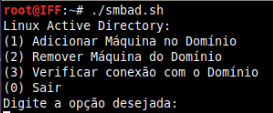
\includegraphics{figuras/smbad}}
   	\caption{Tela do script para inserir maquinas Linux no AD.}
    \label{smbad}
\end{figure}

\section{Compartilhamento de arquivos}

Samba 4 tem um problema com a integração dos usuários e grupos do \textit{Active Directory} com os locais, dificultando a definição das permissões a arquivos e diretórios. Uma solução para tal problema é identificar o código do usuário ou grupo no \textit{Active Directory} e dar as devidas permissões a pasta desejada.

%\begin{itemize}
\noindent \textbf{\# /usr/local/samba/bin/wbinfo "--name-to-sid USERNAME} - O resultado deve ser o sid do usuário no Samba. Exemplo : S-1-5-21-4036476082-4153129556-3089177936-1005 SID\_USER.

\noindent \textbf{\# /usr/local/samba/bin/wbinfo "--sid-to-uid S-1-5-21-4036476082-4153129556-3089177936-1005} - Mostra o id do usuário e é a referência do usuário local com o do Samba 4.

\noindent \textbf{\# /usr/local/samba/bin/wbinfo "--group-info Dtic} - Mostra o gid do grupo e é a referência do grupo local com o do Samba 4.

\noindent \textbf{\# chown 3000011.3000020 /pasta\_que\_será\_compartilhada} - Mudando o usuário do diretório e as suas permissões, o usuário do AD irá ter o acesso aos arquivos.

\section{Windows no domínio Samba 4}

%O procedimento para ingressar um computador Windows no domínio através do Samba 4 é o mesmo executado no caso do Samba 3, porém, no caso do Samba 4 o computador a ser ingressado no domínio não necessita estar cadastrado no servidor pois no momento em que o micro for ingressado no domínio, será automaticamente criada uma conta de máquina com o nome do computador pelo Samba 4.
%Em adição aos procedimentos realizados no Samba 3, para ingressar o computador Windows no domínio pelo Samba 4, deve ser informado o IP do servidor no campo de DNS das configurações de Rede. Para configurar o IP de DNS deve-se:
O procedimento para ingressar um computador Windows no domínio Samba 4 é o mesmo do Samba 3, porém o computador a ser ingressado não necessita ser cadastrado anteriormente, pois o mesmo será cadastrado automaticamente do através do Kerberos.
Em adição aos procedimentos do Samba 3, para ingressar o computador Windows no domínio Samba 4, o DNS do computador deve ser o IP do Samba 4. Para mudar o DNS deve-se:
\begin{itemize}
	\item Acessar as conexões de rede através do Painel de Controle. Figura \ref{conexoes_rede}
	\begin{figure}[h!]
			\centering
	 		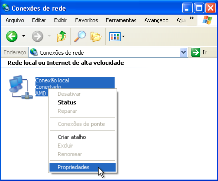
\includegraphics[width=0.5 \textwidth]{figuras/conexoes_rede}
			\caption{Acessando as Conexões de Rede}
			\label{conexoes_rede}
	\end{figure}	
	\item Acessar as propriedades da conexão de rede ativa. Figura \ref{propriedades_conexao}
	\begin{figure}[h!]
			\centering
	 		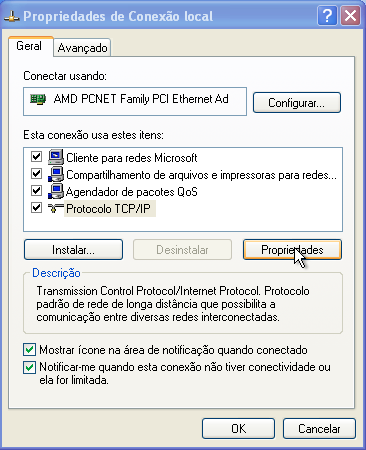
\includegraphics[width=0.4 \textwidth]{figuras/propriedades_conexao}
			\caption{Acessando as propriedades da conexão ativa}
			\label{propriedades_conexao}
	\end{figure}
	
	\pagebreak
	
	\item Incluir o IP do servidor Samba 4 no campo de DNS. Figura \ref{propriedades_tcpip}
	\begin{figure}[ht]
			\centering
	 		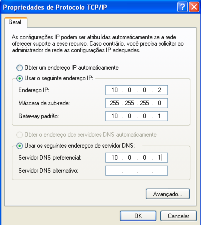
\includegraphics[width=0.5 \textwidth]{figuras/propriedades_tcpip}
			\caption{Incluindo o IP do servidor Samba 4 no campo de DNS}
			\label{propriedades_tcpip}
	\end{figure}
	
	\item Após salvo as configurações, o computador deve ser reiniciado.
	
\end{itemize}